\chapter{基于多粒度切分的局部对齐网络}

\section{引言}
近年来,局部信息在计算机视觉的各种任务中发挥着越来越重要的作用,除了服装图像检索之外,这些任务还包括但不限于:细粒度分类、行人重识别、
视觉问答等。细粒度分类用于在一个大的类别中区分不同的小的类别,比如识别具体的鸟的品种,这需要着重对鸟的一些关键部位(比如嘴巴、眼睛)
做特征学习\cite{wang2018learning};类似的,行人重识别需要抽取行人特定部位(如头部、肩膀、腿部)的信息以消除因姿势不同带来的全局信息的偏差\cite{sun2018beyond};视觉问答任务里,
输入为一幅图像和与这幅图像相关的任何一个问题,算法需要输出这个问题的答案,需要对这幅图有全局的语义理解,同时根据问题侧重的学习相关的局部信息特征。
视觉问答的输入图像一般包括多个实例,输入问题有可能只关注其中的一部分,因此对局部信息的提取可以用目标检测框出所有的实例\cite{anderson2018bottom},而细粒度分类以及
图像检索任务一般涉及单个实例,需要采取不同的策略。

对单个实例的局部信息的学习一般有两种方式:基于软注意力(Soft attention)以及基于硬注意力(Hard attention)。软注意力指对图像不同区域的特征赋予不同大小的权重
,本文第三章提出的网络设计方式就是一种基于软注意力机制的方法,通过学习注意力权重分布图自适应的根据输入调节局部特征的权重以达到对局部信息的抓取,这种方法一般不需要
额外的标注信息去监督;硬注意力本质为软注意力机制的特征形式,软注意力的权重值是连续的(一般为0到1之间),而硬注意力机制则是0——1分布,即只保留部分局部区域的信息,
舍弃其余的信息。基于硬注意力机制的做法一般是通过对原图的切分来实现的,Wei等人提出一种基于关键点的切分方法\cite{wei2017glad},根据关键点所定位出的部件位置
生成检测框,随后再根据检测框对原图裁剪输入网络提取这部分的局部信息,这种方式有一定的有效性,但是需要依赖关键点的标注,对资源消耗较大。Li等提出一种无需额外标注
(只需要类别信息的标签)的切分方式\cite{li2017learning},其做法是直接对输入的图像横向平均切分,将每一个图像切片以及完整的原图送入网络做分类学习,且使用了不同大小的
卷积核对输入进行多尺度信息提取。

本章介绍一种具有创新性的基于切分的局部对齐网络结构,传统的基于切分去学习局部特征的做法大多数是对原图做切分,这种切分方式旨在通过对保留下的局部信息单独训练以达到增强
其语义强度的目的,但是这种直接舍弃大部分图像信息的方式不利于网络收敛,甚至会导致模型的过拟合,基于此弊端提出一种对特征图的切分方式。在此基础上对切分策略做了多方面的
改进,在强化局部特征语义信息的同时做到局部区域更好的对齐。
\section{方法与实现}
所提出的网络框架如图\ref{fig:MGN}所示,输入图像首先经过特征提取器提取特征,此处的特征提取器指基础网络(如ResNet)去除最后的全局池化层以及之后的部分,
输出的特征是一个张量,随后该特征复制若干份,并进入四个并行的分支:Global、Horizontal、Vertical、Annular。其中Global为全局分支,学习全局语义信息,
其余三个分支为局部分支,学习局部特征。
\begin{figure}[h]
  \centering
  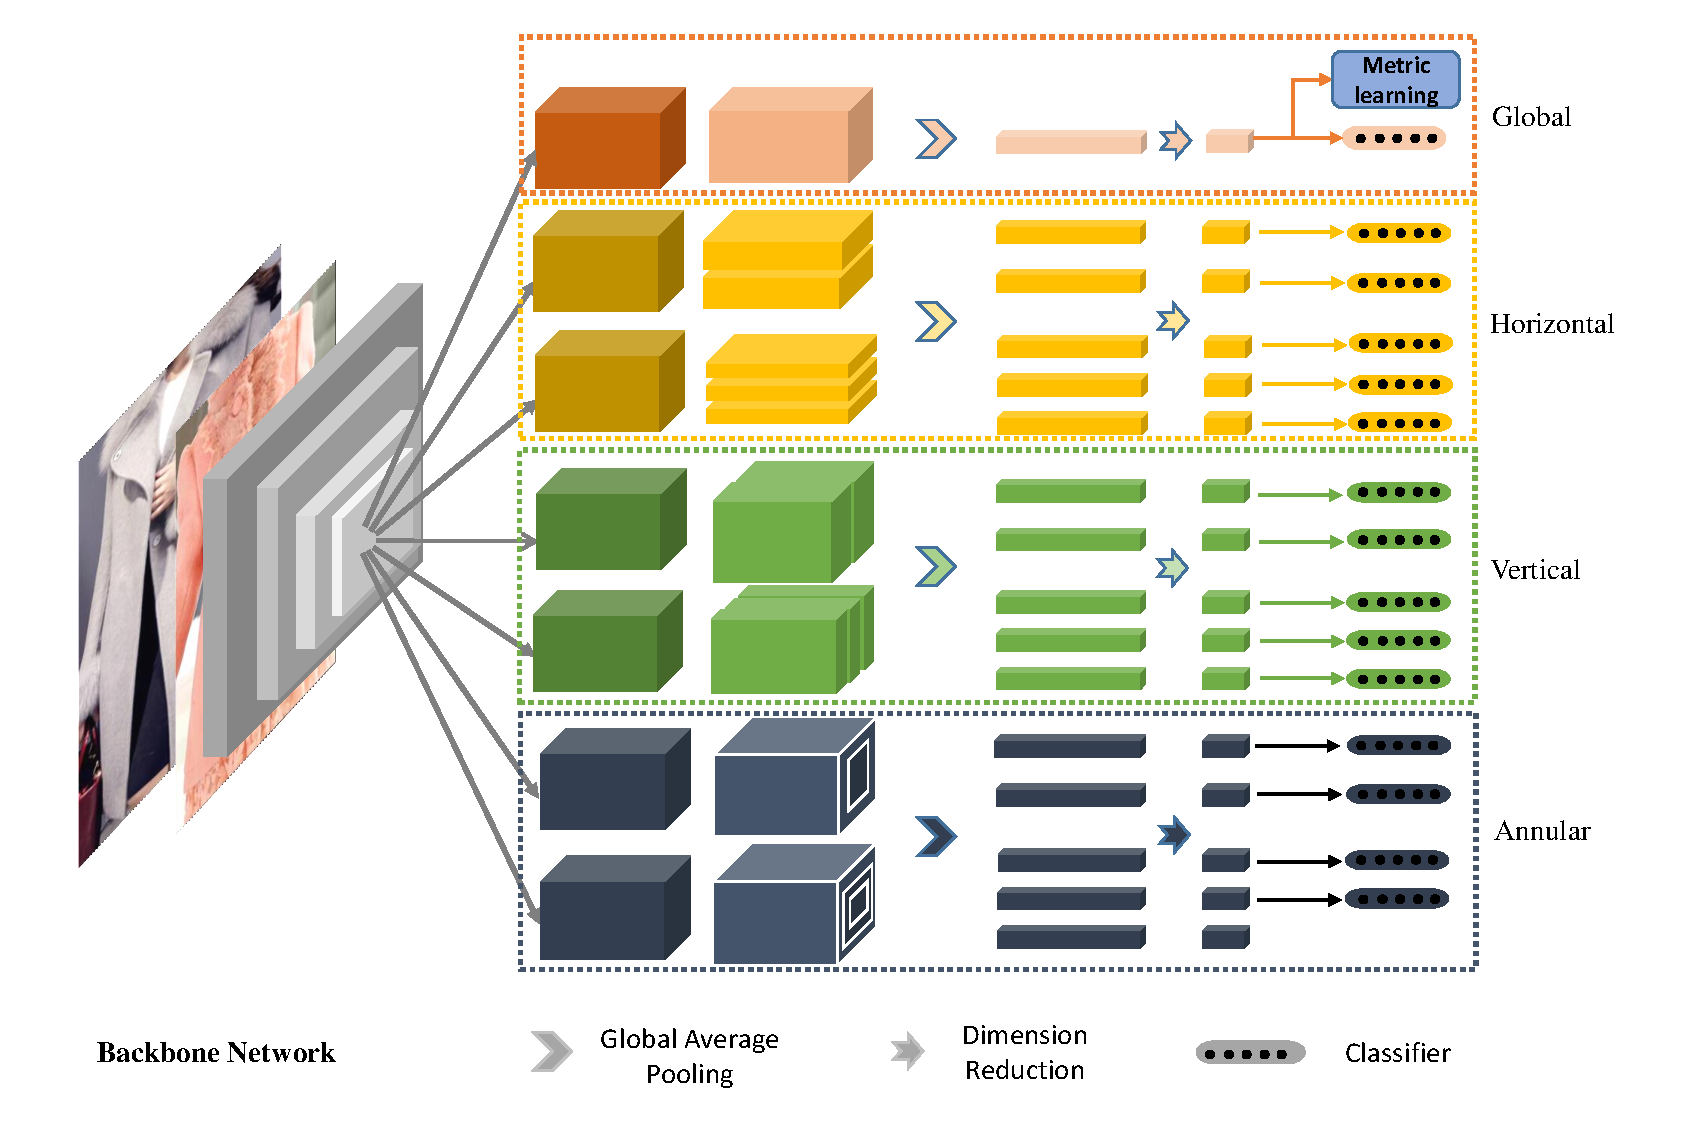
\includegraphics[width=1.0\linewidth]{Img/MGN.pdf}
  \caption{基于切分的局部对齐网络框架图}
  \label{fig:MGN}
\end{figure}

\subsection{对特征图的切分}
传统的基于切分的方式去学习局部特征的做法大多数是对原图做切分,然后将每个图像切片送入网络单独处理,而在本章所提出的方法中,切分操作是对特征图实施,如图\ref{fig:MGN}
中的局部分支所示。我们认为对原图切分之后保留的局部图像切片语义信息不够丰富,直接代表图像去识别其类别可能会导致过拟合,而基于特征图的切分则与之不同,
得益于卷积操作的特性,每个特征切片有着更丰富的上下文信息。
\begin{figure}[h]
  \centering
  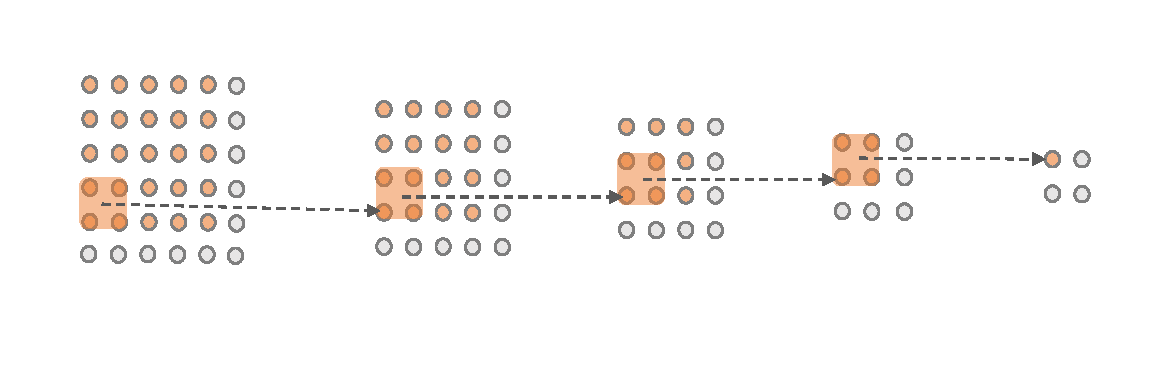
\includegraphics[width=1.0\linewidth]{Img/RF.pdf}
  \caption{卷积操作与感受野}
  \label{fig:RF}
\end{figure}


感受野(Receptive Field)是深度神经网络中的一个很常见的概念,它代表在特征图上的像素点映射到原图后的区域大小。而特征图上某个像素点的感受野的大小并不能按照原图和特征图大小的比例直接计算,
这是由卷积操作的特性所决定的,当前层的感受野与之前所有卷积层的参数都有关系。以图\ref{fig:RF}为例,假设输入图像大小为$6 \times 6$,经过四次卷积层,卷积核大小均为
$2 \times 2$,步长均为$1$,最后得到$2 \times 2$的输出,由图中感受野的变化情况可以看出:最后一层的输出特征图每个像素点对应的感受野对应原图的$5 \times 5$大小区域。

\begin{figure}[h]
  \centering
  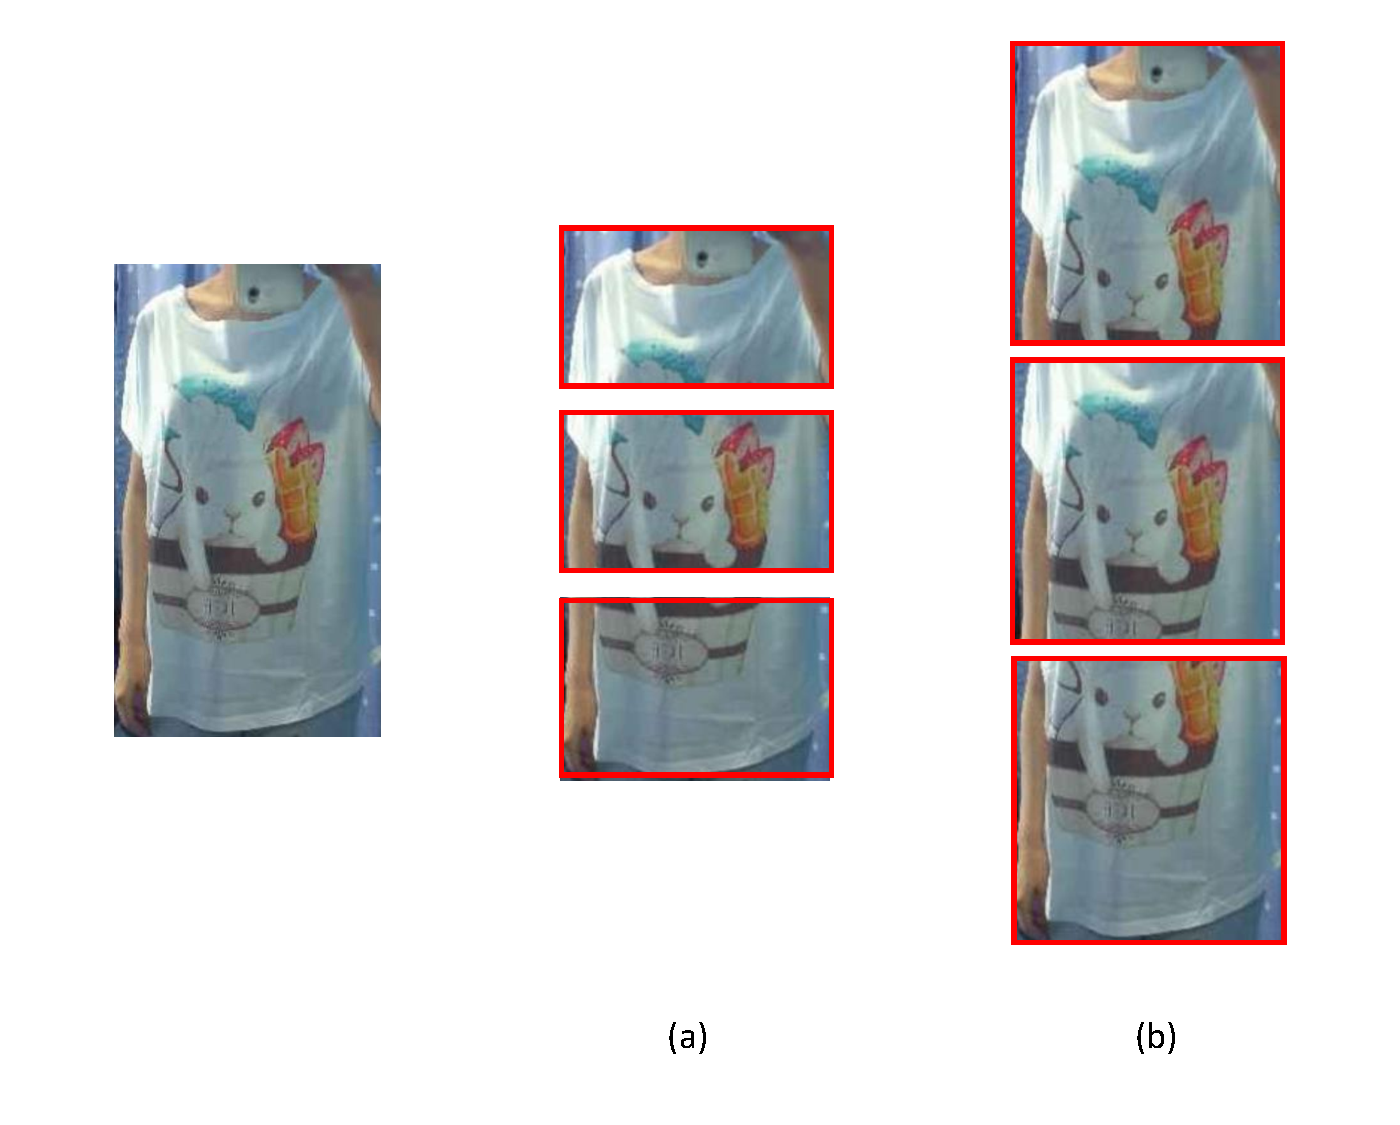
\includegraphics[width=0.8\linewidth]{Img/RFcmp.pdf}
  \caption{对原图切分和对特征切分的理论感受野差别}
  \label{fig:RFcmp}
\end{figure}

上述例子说明对特征图的切分和对原图的切分有根本区别,对特征图切分得到的特征切片包含了原图对应比例区域之外的上下文信息,如图\ref{fig:RFcmp}中,(a)、(b)分别代表
对原图和特征图切分后每个切片对应的理论感受野。然而,以(b)中所示感受野大小为准(有重叠区域)去切分原图和对特征图的切分仍然是不同的,
理论上来说,虽然特征图的每个切片对应的感受野比其在整个特征图所占比例在原图对应区域要大,但是这个区域的信息强度分布并不是平均的。Luo等人指出,卷积神经网络中的理论
感受野与实际感受野有很大差别,实际上来说越是靠近感受野中心的区域信号强度越大,整体呈高斯分布\cite{luo2016understanding}。因此,特征图的特征切片在包含更多的上下文
信息的同时,局部信息可以以相对更强的信号强度表达出来,而直接用有重叠区域的方式对原图切分反而会引入过强的噪音,导致不利于局部信息的表达。

我们对特征提取网络输出的张量进行切分,随后对每个切片进行全局最大池化(Global Max Pooling)得到若干向量,其维度为原特征图的通道数,然后用$1 \times 1$大小的卷积核对这个向量降维,
最后以降维后的向量作为局部特征的表示送入分类器学习原图的类别。分类器对应的损失函数就是Soft Max Loss,这么做的出发点是希望网络可以仅通过输入图像的某个局部区域去区分
其类别,这样可以提高局部区域特征的表达能力。所以,局部分支最后的特征由多个局部切片的向量组成:$\mathcal{F}=\{S_{1},S_{2}\cdots S_{i}\}$,
则该分支的损失为$i$个Soft Max Loss的均值。
\subsection{环形切分}
图\ref{fig:MGN}中,根据对特征切分的实施方式不同,局部分支共有三个:Horizontal(横向切分)、Vertical(纵向切分)、Annular(环形切分)。环形切分是本方法所提出的一种
创新型的切分方式,这三种切分方式的具体实现方式区别如图\ref{fig:annular}所示。图中示例均为三等份的切分,横向或者纵向的切分比较直接,只需在特征图的三等分点进行切割。
环形的切分方式则是按照特征图边缘到特征图中心长度的三等分点,按照“回“字形切分出环形的特征,确切的来说,得到的是外侧的切片为环形、最里侧的切片为矩形的特征。
\begin{figure}[h]
  \centering
  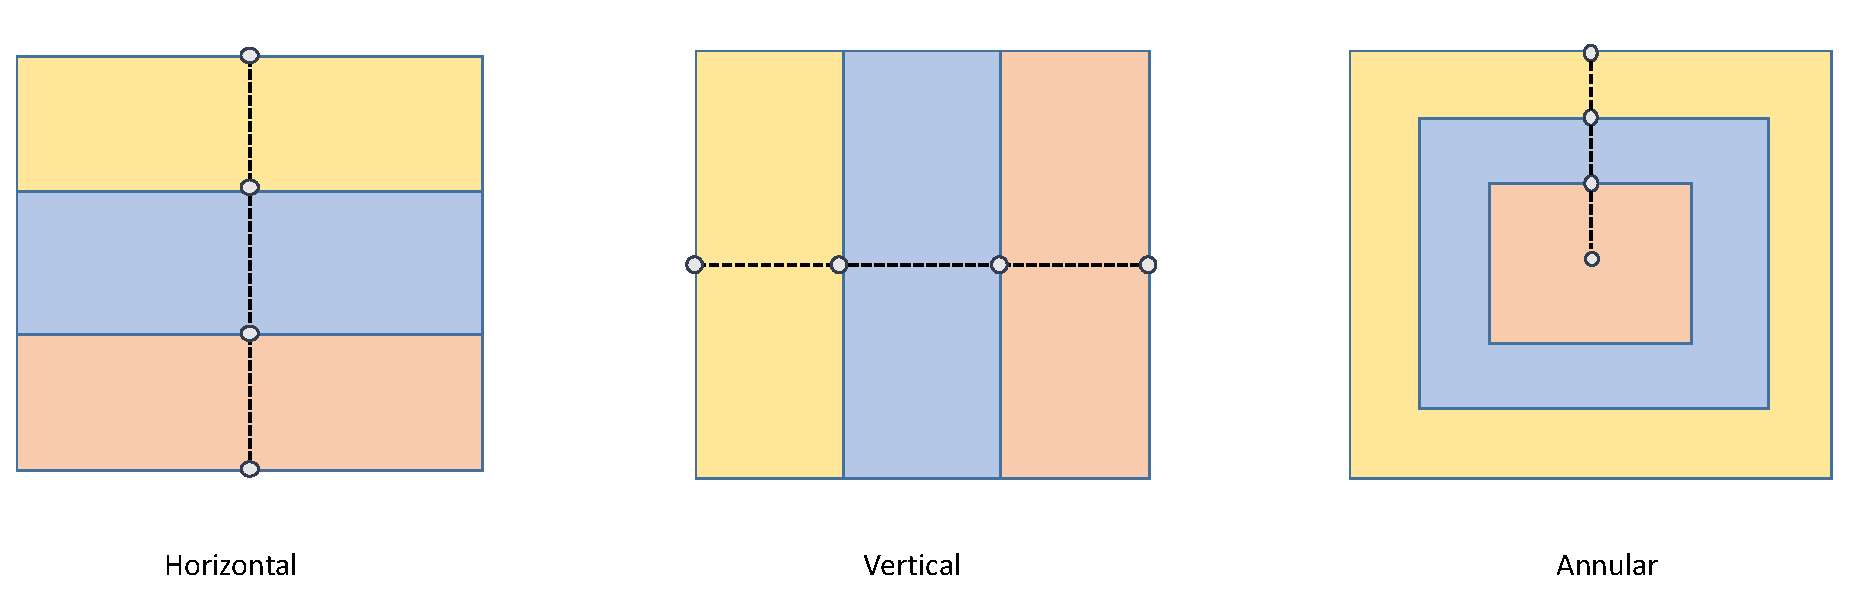
\includegraphics[width=1.0\linewidth]{Img/annular.pdf}
  \caption{对特征图的不同切分方式}
  \label{fig:annular}
\end{figure}


使用环形切分方式的出发点是基于实际场景,服装图像的空间分布多种多样,其中有很多一部分是类似图\ref{fig:annular-vis}中的结构:服装最显著的局部特征位于中心区域,且环形区域内对应有完整的局部区域特性,图中最中心的区域是一个红心的标识,中间的环形有完整的“PLAY”字样,最外的一个环则是衣服领口和袖子的纹理等特性。
这种情况下,横向的切分方式难以保证关键局部信息的完整性,而所提出的环形切分方式可以很好的解决这类问题。此外,环形切分的方式还具有很强的旋转不变性,尤其是对于图像的
中心区域,这种特性可以有效防止图像拍摄的角度偏差所带来的影响,使得模型具有很强的泛化能力。图\ref{fig:annular-vis}中展示了环形切分对旋转因素的有效对抗,原图在旋转
90\degree、180\degree、270\degree 的情况下,环形切分所得到的特征切片的内容不会发生改变,即使在旋转45\degree 的极端情况下,图像的中心区域(也是最显著的局部区域)
的特征切片依然不会有大幅度的改变。
\begin{figure}[h]
  \centering
  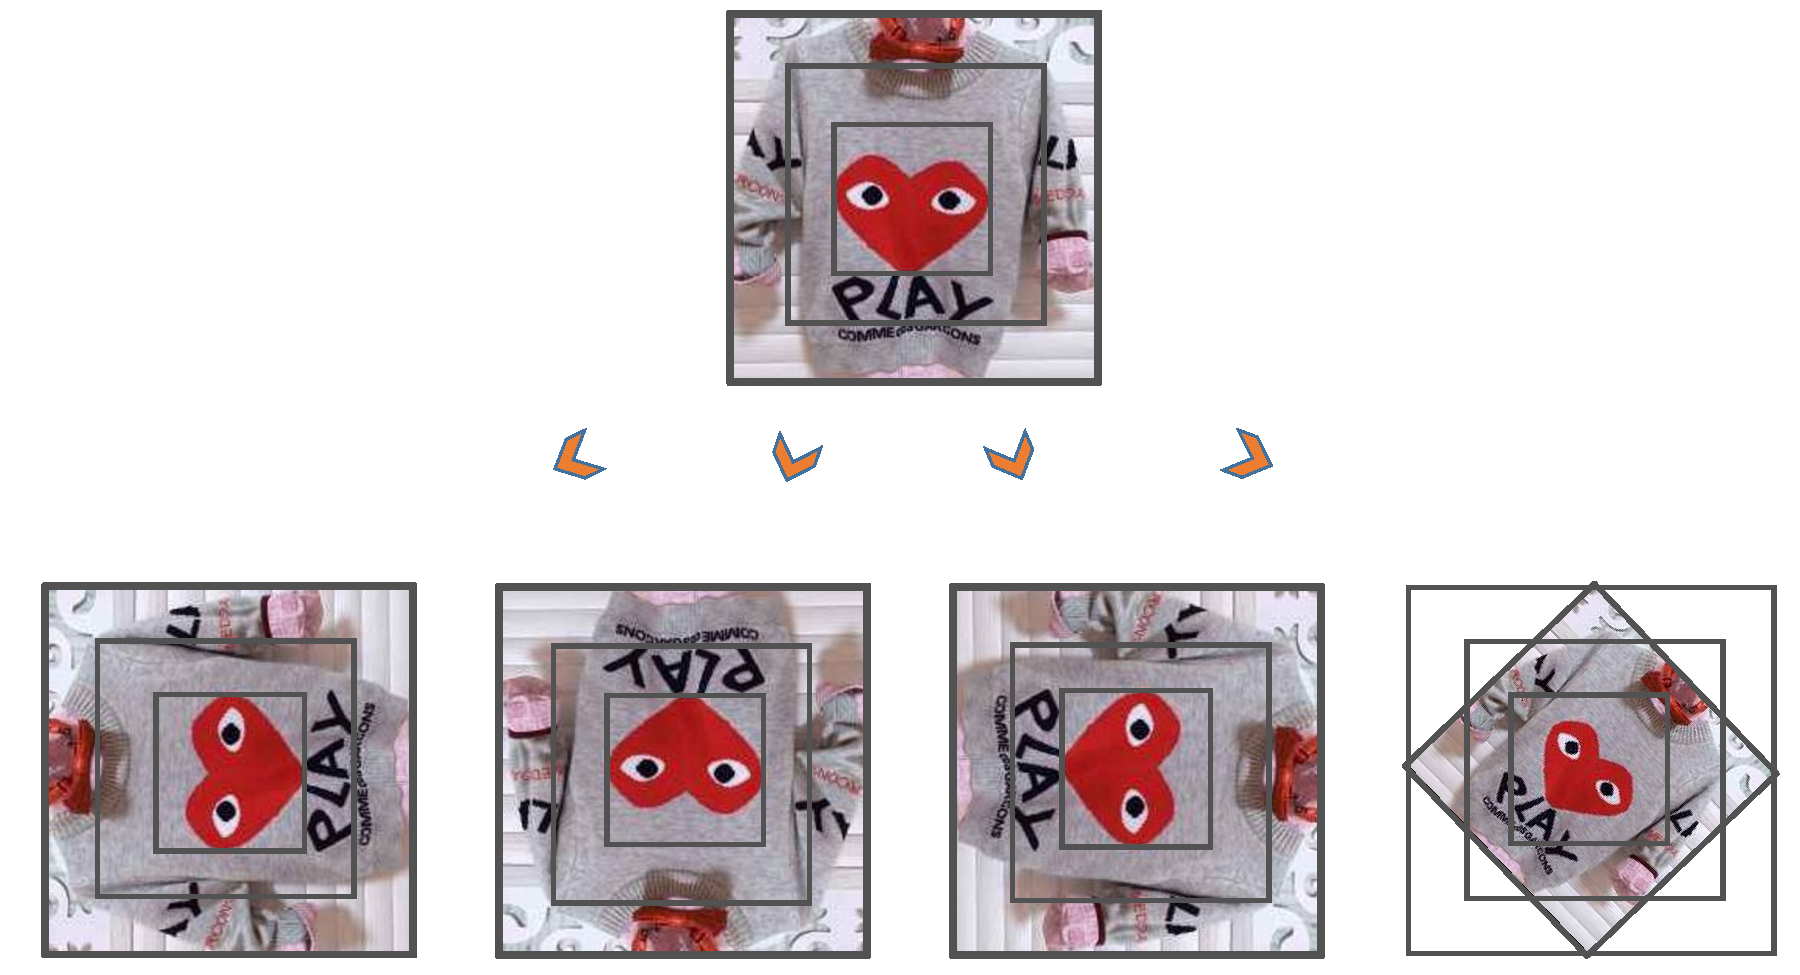
\includegraphics[width=1.0\linewidth]{Img/annular-vis.pdf}
  \caption{环形切分方式的旋转不变性}
  \label{fig:annular-vis}
\end{figure}


此外,横向切分、纵向切分和环形切分的组合方式可以有效提升特征的表达能力。考虑到服装款式的多样性,单一的切分方式不能保证能得到匹配服装图像空间分布的最优特征切片,
而三种切分方式的组合可以对局部特征做更加全面的提取,大大提高了最优特征切片的表达能力,有利于局部区域的对齐。
\subsection{多粒度切分}
本小节介绍一种对特征图使用不同粒度(即多粒度)的切分策略,可以有效提升最终特征的语义表达能力,此处粒度可以理解为尺度或者密度。

\begin{figure}[h]
  \centering
  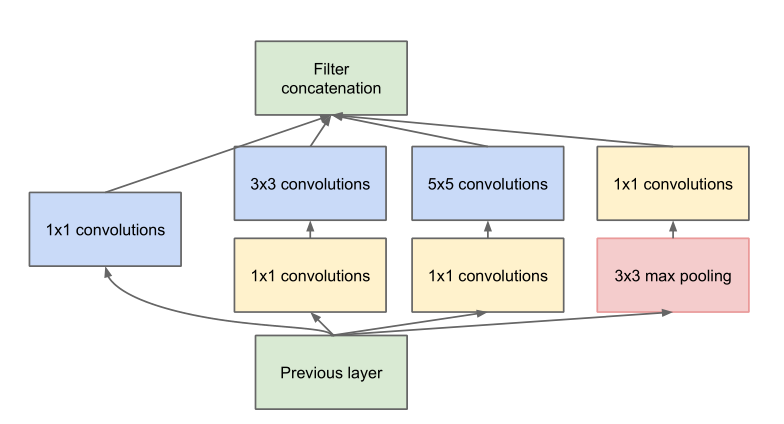
\includegraphics[width=0.75\linewidth]{Img/Inception.png}
  \caption{Inception模块的多尺度卷积}
  \label{fig:Inception}
\end{figure}

本方法受启发于GoogLeNet,图\ref{fig:Inception}描述了GoogLeNet的核心模块的设计方式,对于输入的特征图采用$1 \times 1$、$3 \times 3$、$5 \times 5$三种尺度的卷积核以及一个最大池化层的多路并行分支
提取特征,虽然通过不同的Padding方式可以得到相同大小的特征图输出,但是输出特征的每个像素点对应的感受野却不相同。最后对多个分支的特征图输出在通道维度拼接起来,获得
语义信息更丰富、表达能力更强的特征输出。

类似的网络设计理念还被应用在目标检测和语义分割等领域。目标检测任务中,特征金字塔网络(Feature Pyramid Network, FPN)取得了很大的成功\cite{lin2017feature},其网络设计包含自底向上和自顶向下两个路径
,自底向上即常见的卷积神经网络提取高层语义信息,而自顶向下的过程则是通过上采样逐层放大特征图的分辨率,并且通过阶跃连接和自底向上的特征图融合以修正细节信息,如图\ref{fig:fpn}。最后RPN
层的Anchor取自不同分辨率的特征图。分辨低的层语义信息丰富,有利于大目标的检测;分辨率高的层细节信息丰富,有利于小目标的检测。
\begin{figure}[h]
  \centering
  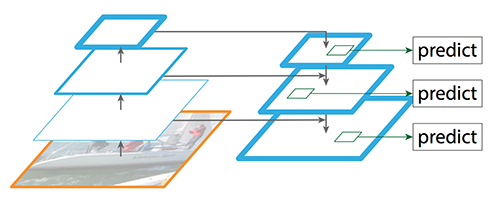
\includegraphics[width=0.75\linewidth]{Img/fpn.png}
  \caption{特征金字塔网络\cite{lin2017feature}}
  \label{fig:fpn}
\end{figure}


所提出的多粒度切分方法对特征图按照不同的密度(尺度)切分,不同的切分粒度可以得到不同大小的特征切片,他们所包含的语义信息也有所区别,这些特征切片分别输入分类器进行
分类训练。在测试阶段,这些感受野不同的局部特征切片拼接为一个整体(池化以后的向量),融合了不同尺度的局部特征信息,获得更强的表达能力。图\ref{fig:sg-mg}以横向切分
为例对比了单粒度切分与多粒度切分在实施时的区别,图中每个虚线框框出的部分代表一种切分粒度,且每个虚线框的输出都是由相同的特征图复制得到
,不同的切分粒度对应不同数量的特征切片数目。理论上来说,不同切分粒度的数量没有限制,但是不同的切分粒度带来更多的特征切片,这也会导致最终拼接的特征维度变得很高
,所以需要在模型性能和特征维度之间作出权衡。
\begin{figure}[h]
  \centering
  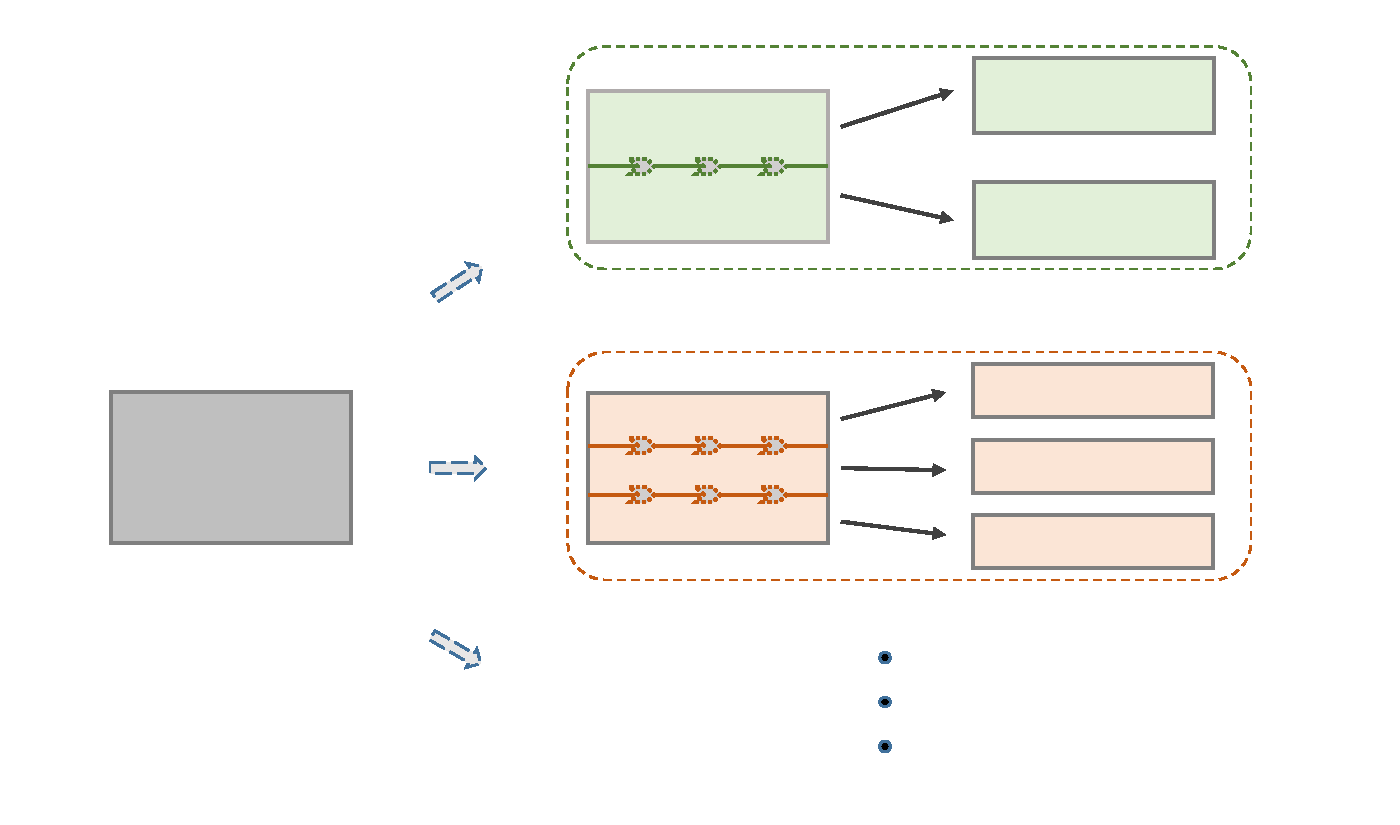
\includegraphics[width=1\linewidth]{Img/sg-mg.pdf}
  \caption{单粒度切分与多粒度切分的对比图}
  \label{fig:sg-mg}
\end{figure}

\section{实验与分析}
本章节实验设定与第三章基本相同,特征提取网络选择SE-Inceptionv2,模型在DeepFashion数据集上训练,在ALISC2015数据集测试。模型性能的评价指标为query检索结果top 4的准确率,即每个query的top 4检索结果中
若至少有一个和query是同款服装,则这个query检索成功。训练和测试数据同样需要目标检测进行预处理,DeepFashion提供了检测框的标注可以直接用于裁减,ALISC2015并没有提供
框的标注,要通过Faster R-CNN检测器对上装、下装和群装进行检测框的预测,且遵循每幅图最多保留一个检测框的准则。
\subsection{基于特征图的切分}
% Table generated by Excel2LaTeX from sheet 'ablations'
\begin{table}[ht]
  \centering
  \caption{对图像切分以及对特征图切分的对比实验}
   \setlength{\tabcolsep}{6mm}{
    \begin{tabular}{l|ccc|c}
    \hline
    实验 & 上装 & 下装 & 群装 \\\hline
    \hline
    Baseline & 74.8  & 71.3  & 64.0  \\
    Image-2p & 75.0  &  71.3 & 64.2  \\  
    Image-Overlap-2p& 74.8 & 69.0 &64.5 \\
    FeatureMap-2p& 78.3&75.1&67.7 \\
    Image-3p & 75.6  &  71.5 & 64.8  \\  
    Image-Overlap-3p& 75.0 & 71.0 &63.9 \\
    FeatureMap-3p& 80.1&77.3&\textbf{69.1} \\
    Image-4p & 75.2  &  70.7 & 64.2  \\  
    Image-Overlap-4p& 73.6 & 71.0 &62.4 \\
    FeatureMap-4p $\star$& \textbf{80.3}&\textbf{77.8}&\textbf{69.1} \\
    Image-5p & 73.8  &  68.8 & 63.3  \\  
    Image-Overlap-5p& 73.4 & 68.5 &62.0 \\
    FeatureMap-5p&\textbf{80.3}&77.5&68.7 \\
    \hline
    \end{tabular}%
    }
  \label{tab:featuremap}%
\end{table}%


表\ref{tab:featuremap}详细讨论了对特征图切分和对原图切分对模型性能的影响。表中Baseline指对特征提取网络输出的特征全局平均池化后降维作为图像最后的表示,送入分类器训练。
主要对比了:对原图切分且不同切片之间无重叠区域(Image)、对原图切分且不同切片之间有一定重叠区域(Image-Overlap)、对特征图切分(FeatureMap)三种切分方式,其中-$n$p
代表切分后的切片数目(p代表part,Image-Overlap-3p代表对原图有重叠的切分为三等份),表中的实验结果均采用横向切分。全面分析这些结果后我们可以得到如下结论:
\begin{itemize}
  \item[1.]对原图有重叠的切分方式(Image-Overlap)训练模型会得到比Baseline更低的结果。
  \item[2.]对特征图切分(FeatureMap)的效果显著,切分为两个part就可以得到比Baseline高2到3个点的结果。对原图无重叠的切分在切片数目较小时相比较Baseline也有一定的提升,
    但随后也会得到低于Baseline的结果。整体而言不同切分方式对应的模型性能比较为:FeatureMap > Image >Image-Overlap。
  \item[3.]在对原图切分的切片数较大时(4个或5个),有无重叠区域对模型的性能影响不大,且效果都比较差。
  \item[4.]对特征图的切分方式随着切分粒度的逐渐细化,模型的性能呈现上升后平稳或者略微下降的趋势,性能最优的一组实验为对特征图切分4均份。
\end{itemize}

表中$\star$表示当前消融实验最优的实验设置,这组实验的设置也会作为下一组实验的Baseline。
\subsection{环形切分}
本小节探究环形切分以及不同切分方式的组合是否对模型的表达能力带来提升,表\ref{tab:annular}展示了对三种切分方式单独使用以及三种方式组合的结果。实验表明,纵向切分要比横向切分
效果略差,这是因为横向切分出的局部区域信息结构性更强,符合服装设计的实际情况。环形切分的方式和横向切分性能相当,甚至有微弱的提升,这个结果充分证明了环形切分的策略
对局部特征的提取更具优势。最后一组实验采用多个分支的方式,即横向、纵向和环形三个分支,每个分支均切分为4等份,最终得到了最好的效果,且提升较为可观。从表\ref{tab:featuremap}
中可以看出,单纯的增加part的个数并不会带来模型性能的提升(在大于4之后稳定),而三种切分方式的组合得到了12个part,同时进一步提升了性能,这说明不同的切分方式带来了
更加充分的局部语义信息。
% Table generated by Excel2LaTeX from sheet 'ablations'
\begin{table}[ht]
  \centering
  \caption{环形切分与组合式切分的有效性分析}
   \setlength{\tabcolsep}{6mm}{
    \begin{tabular}{l|ccc|c}
    \hline
    实验 & 上装 & 下装 & 群装 \\\hline
    \hline
    Horizontal(Baseline) & 78.3&75.8&67.1 \\
    Vertical & 77.7  &  75.5 & 65.9  \\  
    Annular & 78.8 & 76.0 &66.9 \\
    Horizontal+Vertical+Annular $\star$& \textbf{79.4}&\textbf{76.6}&\textbf{67.7} \\
    \hline
    \end{tabular}%
    }
  \label{tab:annular}%
\end{table}%


\subsection{多粒度切分}
在表\ref{tab:mg}中,我们对比了单粒度(SG,Single Granularity)与多粒度(MG,Multi Granularity)的切分效果,并且探究了不同的切分粒度组合。以上一组实验中的三个分支
(对应横向、纵向、环形三种切分方式),每个分支切分为四份的设定作为Baseline,共$4 \times 3$个part。在多粒度的实验中,($m + n$)表示使用$m$和$n$两种切分粒度的
组合。
% Table generated by Excel2LaTeX from sheet 'ablations'
\begin{table}[ht]
  \centering
  \caption{多粒度切分的有效性分析}
   \setlength{\tabcolsep}{6mm}{
    \begin{tabular}{l|cccc|c}
    \hline
    实验 & Part个数 & 上装 & 下装 & 群装 \\\hline
    \hline
     SG / $4\times3$(Baseline)&12&79.4 &76.6&67.7 \\
     SG / $5\times3$      & 15  & 79.4 &76.2&67.9 \\
     MG / $(2+3)\times3$  & 15  & \textbf{80.2} & \textbf{77.1} &68.8 \\
     MG / $(3+4)\times3$  & 21  & \textbf{80.2} &76.9&69.0 \\
     MG / $(2+3+4)\times3$& 27  & \textbf{80.2} & \textbf{77.1} & \textbf{69.3} \\
    \hline
    \end{tabular}%
    }
  \label{tab:mg}%
\end{table}%


分析这几组对比试验我们可以得出如下结论:
\begin{itemize}
  \item[1.]在单粒度切分的设定下,简单的增加每个分支的part个数(4个变为5个)并不会带来性能上的提升。
  \item[2.]对比SG / $5\times3$和MG /(2+3)$\times3$可以发现,在part总数量相同的情况下,多粒度组合的切分方式相较单粒度的切分方式在三个服装类别都有接近1个点的提升。
    这也充分说明多粒度切分方法的有效性。
  \item[3.](3+4)和(2+3+4)的粒度组合可以进一步提高模型性能,但是都比较微弱,而且随着part数目的增加,拼接后的特征维度也会变大进而影响检索速度。综合考虑,
    取(2+3)作为本方法的最优设定。
\end{itemize}
\subsection{对池化方式与特征维度的探讨}
如上文所提及的,我们取SE-Inceptionv2最后的全局平均池化(GAP,Global Average Pooling)层之前的部分作为特征提取器,并对得到的张量进行后续的操作。通常来讲,特征提取网络会保留最后的全局平均池化层,
输出一个向量,这是因为GAP可以很好的表达全局的语义信息。而我们所提出的对特征图的切分方法旨在提取局部区域的特征,切分得到的每个part代表一个局部区域,局部区域往往更注重
个别关键像素点的特征表达,因此我们考虑对每个part采用全局最大池化(GMP,Global Max Pooling)。

最大池化操作具有平移、旋转不变性的特性,这也非常有利与更好的去除part中的噪声,池化之后只保留每个part最为显著的特征值,基于这个假设,我们对不同的池化方式做了对比试验
。相关结果如表\ref{tab:pooling}所示,试验表明最大池化在上装和下装两类的表现要比平均池化更好,我们融合平均池化和最大池化的结果(GAP+GMP,对得到的向量相加)得到了最好的一组结果,
这说明对局部区域进行最大池化得到的特征的确是有益的。
% Table generated by Excel2LaTeX from sheet 'ablations'
\begin{table}[ht]
  \centering
  \caption{对part平均池化与最大池化的效果对比}
   \setlength{\tabcolsep}{6mm}{
    \begin{tabular}{l|ccc|c}
    \hline
    实验 & 上装 & 下装 & 群装 \\\hline
    \hline
     GAP & 82.2 & 79.1 & 71.3 \\
     GMP & 82.5 & 79.3 & 70.4 \\
     GAP+GMP $\star$ & \textbf{83.3} & \textbf{79.7} & \textbf{71.5} \\
    \hline
    \end{tabular}%
    }
  \label{tab:pooling}%
\end{table}%

% Table generated by Excel2LaTeX from sheet 'ablations'
\begin{table}[ht]
  \centering
  \caption{每个part特征维度对模型性能的影响}
   \setlength{\tabcolsep}{6mm}{
    \begin{tabular}{l|ccc|c}
    \hline
    维度 & 上装 & 下装 & 群装 \\\hline
    \hline
     128  & 81.9 &  79.4 &  70.6 \\
     256 $\star$ & 83.3 &  \textbf{79.7} &  71.5 \\
     512  & \textbf{83.5} &  \textbf{79.7} & \textbf{71.9} \\
    \hline
    \end{tabular}%
    }
  \label{tab:mgn-dim}%
\end{table}%


网络在池化层之后,接了一个$1\times1$的卷积层对每个part的特征降维,在上述所有实验中,我们取256维作为默认输出维度。现在我们单独对维度的参数进行了实验对比,如表\ref{tab:mgn-dim},表中维度代表每个part的维度。
实验结果表明,每个part维度由256降至128时有1个点左右的下降,升至512时有微弱的提升。权衡性能和特征大小,取每个part输出256维特征作为默认设定。

\subsection{全局特征与局部特征的结合}
以上几个小节通过对不同方法和超参的探讨,确定了局部对齐分支(Horizontal、Vertical、Annular)的设计方式。而最终的网络结构如图\ref{fig:MGN}所示,除了局部对齐的分支以外
,还有一支全局(Global)的分支,从图中可以看出,对比三个局部分支,Global分支还引入了度量学习,即Triplet loss。

% Table generated by Excel2LaTeX from sheet 'ablations'
\begin{table}[ht]
  \centering
  \caption{全局信息与局部信息的结合}
   \setlength{\tabcolsep}{6mm}{
    \begin{tabular}{l|ccc|c}
    \hline
    实验 & 上装 & 下装 & 群装 \\\hline
    \hline
     Local  & 83.5 &  79.7 &  71.9 \\
     Local+Global(without triplet loss)& 84.6 & 80.3 &  73 \\
     Local+Global(with triplet loss) $\star$  & \textbf{85.2} &  \textbf{80.5} & \textbf{74.1} \\
    \hline
    \end{tabular}%
    }
  \label{tab:global-local}%
\end{table}%

相应的实验如表\ref{tab:global-local}所示,全局特征与局部特征的结合对模型性能很有帮助,且度量学习在检索任务的有效性再次得到验证。事实上,我们尝试将Triplet loss加入
每个part的监督之中,但是得到了非常差的效果,我们推测度量学习较为适用于对样本全局信息的学习,而某些part包含较大量的噪声信息,用Triplet loss做监督不利于模型收敛。

\section{本章小结}
本章提出一种基于对特征图切分的局部对齐网络,实验证明对特征图的切分对比对原图的切分方式有很大优势。采用多种切分方式的组合(横向、纵向、环形)有效增大保留关键局部区域信息
完整性的可能,有利于局部区域的对齐。提出多粒度的切分策略,这种类似特征金字塔的结构利用不同的感受野包括了不同尺度的局部信息,有效提高了输出特征的表达和泛化能力。
此外,针对局部区域的特征提出创新型的池化方式,有效结合最大池化和平均池化的优势。最后,结合全局和局部信息,并引入度量学习,进一步提升网络性能。
